\chapter{Content retrieval}
\label{retrieval}

In order to analyse sentiment on Twitter, the first problem posed is how exactly we retrieve the necessary data for analysis. In essence there are two types of data we need, Twitter data for labelling in order to train our system and a much larger set of Twitter data to classify, in order to better understand sentiment on Twitter. We will draw these two slightly disparate elements together under the banner of content retrieval, as although their intended use is quite different, the two types of data share many similarities both in the way they are collected and stored. Once collected the data must then be prepared either for training or classification. This chapter shall first examine the Twitter APIs relevant to this project along with how they are accessed and used. It will then go on to discuss any pre-processing which takes place, before going on to discuss how we label and annotate our data. Lastly we shall evaluate the success of the system in our evaluation section.

\section{Data structure and storage}
\label{retrieval:data}

As described above, information regarding statuses\footnote{We will use the terms \emph{status} and \emph{tweet} interchangeably throughout this project to refer to the same concept. Not only do Twitter use the term status within their object model, but it is also semantically more accurate for this project which eventually hopes to classify statuses from a variety of micro-blogging services.} serves two purposes within this project, firstly when labelled it can serve as training data, and if unlabelled, it can be classified by our sentiment analysis engine in the hope of better understanding the overall opinion and emotion on Twitter. Essentially this means that every status retrieved can be expanded upon with additional information pertaining to both an annotator and-or classifier's decisions as to its sentiment labels. Throughout this project we shall use MongoDB as our primary data store, both for reasons we shall give throughout the rest of this chapter and those outlined in chapter \ref{background}. Although MongoDB does not require that documents added to it adhere to any schema, the requirements of our project insist that the basic attributes illustrated in listing \ref{retrieval:example_json_tweet} are present. Both \texttt{trained\-\_status} and \texttt{classified\-\_status} are optional additional attributes.

\begin{lstlisting}[language=Ruby, caption={Basic JSON structure for status objects stored in MongoDB}, label=retrieval:example_json_tweet]
{
	"text" : "Hi, this is an example tweet!"
	"source" : "search_api" | "streaming_api"
	"source_id" : NumberLong("78133750344597504"),
	"posted_at" : "Tue Jun 07 2011 17:18:46 GMT+0100 (BST)",
	"from_user" : "joeroot"
	"trained_status" : {
		"subjectivity" : "subjective" | "objective" | "spam"
		"polarity" : "positive" | "negative" | "neutral"
	}
	"classified_status" : {
		"subjectivity" : "subjective" | "objective" | "spam"
		"polarity" : "positive" | "negative" | "neutral"
	}
}
\end{lstlisting}

In order to express this JSON structure within Ruby, we will create three new classes, \emph{Status}, \emph{TrainedStatus} and \emph{ClassifiedStatus}. The core status class will consist of all the attributes described within our JSON schema (listing \ref{retrieval:example_json_tweet}), along with attributes for retrieving a \emph{Status}'s relevant training or classification data. Both the \emph{TrainedStatus} and \emph{ClassifiedStatus} classes will maintain the \emph{Status} class' original attributes, along with new ones for accessing any relevant label data. As shown in figure \ref{fig:status_uml}, both \emph{TrainedStatus} and \emph{ClassifiedStatus} inherit attributes from their parent \emph{Status} class.

\begin{figure}[h!]
	\caption{Class structure for representing tweets/statuses}
	\label{fig:status_uml}
	\centering
	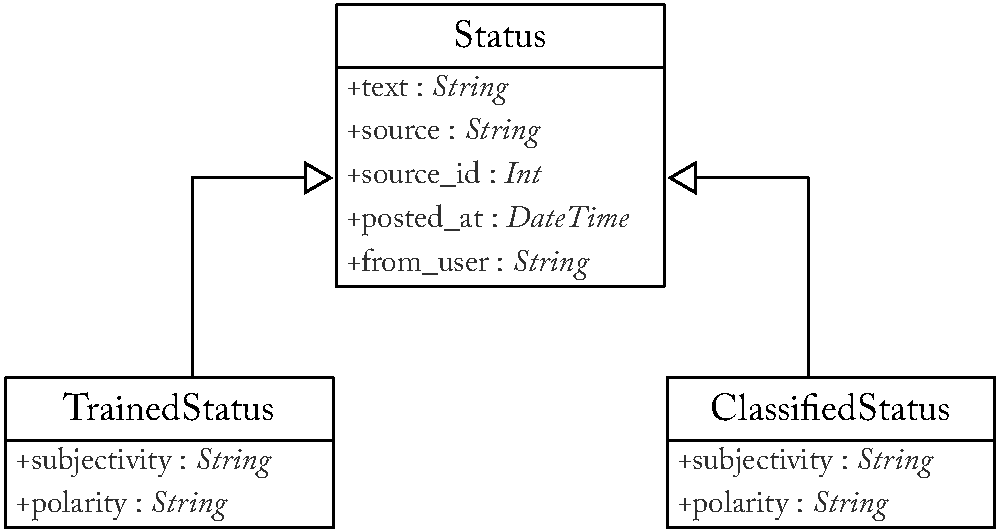
\includegraphics[width=0.83\textwidth]{figures/status_uml_class_diagram.pdf}
\end{figure}

As we go on to explore other components in later chapters, we will add and expand upon this initial core set of attributes and methods. 

The simplicity of MongoDB means any additional data which might be discovered regarding tweets can be inserted as new attributes without any schema worries. In order to map our MongoDB data to Ruby classes we have used an open-source library called \emph{MongoMapper}. MongoMapper gives us the ability to map class objects and attributes to documents within MongoDB. This means that rather than loading and storing an object's attributes in memory, MongoMapper will always read and write directly to the relevant database document. Listing \ref{retrieval:status_code} demonstrates how this mapping is setup for the \emph{Status} class.

\section{Retrieving content on Twitter}

Twitter offers three core APIs for accessing their data, all of which return the said data in either JSON or ATOM format. The three APIs offered are:

\begin{description}
	\item [REST API] - Twitter's REST API provides direct access to Twitter's data model. Requests can be made to access a wide variety of Twitter data, such as user information, timelines, statuses and trends. Essentially Twitter makes all of their sites functionality available through it's API.
	\item [Search API] - Twitter's search API makes their internal status search engine available to developers. Given a query and set of parameters, the search API will find all relevant statuses and return them in the requested format. The status objects returned contain less information than those in the REST API.
	\item [Streaming API] - Twitter's streaming API grants developers access to a high-throughput near-realtime percentage of Twitter's live data. In general Twitter makes 1\% to 10\% of all statuses available through the API and includes further methods for filtering by keywords.
\end{description}

This project shall make use of the \emph{search} and \emph{streaming} APIs. The search API will be used to find tweets for labelling whilst the streaming API shall be employed to collect and filter data for classification. As noted in section \ref{retrieval:data}, data is stored in MongoDB as JSON objects, thus all API calls will request that results be returned in JSON.

\subsection{Search API}

Twitter's search API allows developers to search for tweets matching a specified set of criteria. This is made available through a web-based API, accessible by making GET requests to \texttt{http://\-search\-.\-twitter\-.\-com\-/\-search\-.\-json}. Parameters can be passed to the API through the request headers. For example appending \texttt{q=\-david\-\%20cameron} to the request headers would prompt the API to search for all statuses containing the words "david" and "cameron". Twitter formats the returned data as JSON, with the search results being stored as an array of tweets in the \texttt{results} variable, as demonstrated in listing \ref{retrieval:example_search}.

In order to search and store Twitter data, we created a singleton \emph{TwitterSearch} class. It's \texttt{search} method takes a query string and a parameters hash\footnote{It is common practise amongst Ruby developers to use a \emph{parameters hash} for passing in optional methods to a method. The hash is declared last in a method's arguments, and can be left out when calling the method. If left out, the method definition ensures that the parameters hash is instantiated as an empty hash to prevent any \texttt{nil} errors.}. The parameters hash is used to pass in optional arguments, which map directly to Twitter's search API's optional arguments. Optional parameters include restricting tweets to certain languages through the \texttt{locale} parameter or the \texttt{until} parameter for finding tweets up to a specified date. The query string and parameters are then combined to generate a request URL. Once generated, the \texttt{open-uri} library is used to make a GET request to the URL, and the returned JSON data is stored in a local variable for formatting. Each result's JSON data is amended with a \texttt{source} attribute to identify that the status was retrieved using the Twitter search API. The remaining JSON data however is left unchanged and intact. Once amended, each result is initialised as a \emph{Status} object using it's JSON data. When initialised, MongoMapper automatically writes the data to MongoDB for later use, thus all results are persisted within our database.

Although there are plenty of Ruby libraries available for accessing Twitter's search API, they are often bloated. Many implement their own class structure for representing Twitter's object model which is both unhelpful and unnecessary for this project. Furthermore, although some offer cacheing, none provide support for database persistence. Instead our choice of MongoDB and MongoMapper mean that simply through retrieving the JSON results and using them to initialise \emph{Status} objects, we will have persistent access to the results. 

\subsection{Streaming API}

Twitter's graded streaming APIs deliver developers realtime Twitter data. The three grades, \emph{spritzer}, \emph{garden-hose} and \emph{fire-hose} offer different volumes, ranging from 1\% to 100\% of all realtime tweets. This project shall utilise the \emph{garden-hose} level, which delivers between 1\% and 10\% of all live statuses. Furthermore Twitter offer API methods for filtering the stream ensuring that only tweets matching an array of keywords are included. Twitter make this available by opening an HTTP connection, but never closing it. Tweets are then passed down this connection to the developer. The method call is made to \texttt{http://\-stream\-.twitter\-.com\-/1\-/statuses\-/fi\-l\-ter\-.json} using the \texttt{track} parameter to pass in the set of keywords. For example appending \texttt{track=nhs,david\%20cameron} to the request header will filter the stream for all tweets containing "nhs" or "david cameron". The results are formatted as JSON with each result being separated by a line break. The returned data is slightly more detailed than that returned by the search API, however the core data still adheres to the same schema.

\section{Pre-processing}
\label{subjectivity:pre-processing}

Pre-processing hopes to determine the linguistic attributes of a status which have not already been computationally identified. Primarily we are interested in identifying any grammatical meta-data, in this case each word's part of speech tag, along with any Twitter meta-data the word might contain such as hashtags and mentions. Although not necessarily features themselves, this additional detail will help better describe the data and thus prove useful when building features which truly understand the linguistic nature of Twitter statuses.

\subsection{Part of speech tagger}

Numerous approaches have been taken to part-of-speech tagging, however for the purpose of this project we will implement a Ruby adaptation of Coburn's Perl part of speech tagger\footnote{http\-://\-search\-.cpan\-.org\-/~\-acoburn\-/Lingua\--EN\--Tagger}. Coburn's approach is dependant upon a large corpora of text, within which each word has been annotated with its part of speech tag. For each word within the corpora, we calculate the probability of it being used as a certain part of speech, given by how often it occurs as that said part of speech. For example, if the word \emph{like} appears twice as a an infinitive verb, and once as a past tense verb, the probability of it being an infinitive verb will be $\frac{2}{3}$, and the probability of it being a past tense verb will be $\frac{1}{3}$.

\begin{equation}
	\Pr(tag \mid word) = \frac{|\occurences(word \text{ as } tag)|}{|\occurences(word)|}
\end{equation}

Once this is done, we then use the corpora to calculate the probability of a tag occurring, given the previous word's tag. For example, if an infinitive verb is followed by a proper noun twice and an adjective once, then the probability of a word being a proper noun given the word before it was an infinitive verb is $\frac{2}{3}$, and the probability of it being an adjective is $\frac{1}{3}$.

\begin{equation}
	\Pr(tag \mid tag_{p}) = \frac{|\occurences(tag_{p} \text{ preceeding } tag)|}{|\occurences(tag_p)|}
\end{equation}

Thus, when determining a word's part of speech tag, we want to find the tag which maximises the product of the two probabilities, given our current word and the part of speech tag for the word which preceded it.

\begin{equation}
	\label{eqn:pos}
	\pos(word,tag_{p}) = \argmax_{tag \in tags} (\Pr(tag \mid word) \cdot \Pr(tag \mid tag_{p}))
\end{equation}

Our \emph{TweetTagger} class replicates the above behaviour in Ruby. Colburn's pre-trained probabilities are stored in two separate text files and read into two hashmaps when a \emph{TweetTagger} object is instantiated. In order to tag a body of text with it's appropriate part of speech tags, we can call the \texttt{fetch\_tags(text)} method, passing in the body of text we wish to tag as a parameter. Before we tag the text, it is first split on it's white space and punctuation, using our \texttt{split(text)} function, as demonstrated in listing \ref{overview:example_split_function}.

\begin{lstlisting}[language=Ruby, numbers=none, caption={Example use of split function}, label=overview:example_split_function]
TweetTagger.new.split("Hello, please split this string.")
	=> ["Hello", ",", "please", "split", "this", "string", "."]
\end{lstlisting}

Once split, we are able to tag each word and punctuation mark with it's appropriate part of speech tag. This is done through the \texttt{assign\_tag\-(word\-, \-previous\_tag)} method, a Ruby implementation of equation \ref{eqn:pos}. Where a word does not exists within our lexicon of trained probabilities, and thus no probability score can be calculated for it, it is passed on to the \texttt{unknown\_word\-(word)} method. This attempts to find the word elsewhere, and will be of particular use when adapting the tagger for use on Twitter statuses, and is discussed in detail in section \ref{retrieval:pos_statuses}. For now however, we will assume it manages to find the correct tag.

Once every word has been tagged, the \texttt{fetch\_tags(text)} method returns a JSON formatted, ordered array of words and their corresponding tags. For example, if we were to call \texttt{fetch\_tags} with \emph{Example 1}, the returned JSON would be as shown in listing \ref{overview:example_1_pos_json}.

\begin{lstlisting}[language=Ruby, numbers=none, caption={Returned part of speech tags for \emph{Example 1}}, label=overview:example_1_pos_json]
TweetTagger.new.fetch_tags("I think David Cameron is doing a rather good job: strong leader, holding together seemingly impossible coalition, keeping labour at bay")
	=>	[{"word" : "I", "tag" : "prp"}, {"word" : "think", "tag" : "vbp"}, {"word" : "David", "tag" : "nnp"}, {"word" : "Cameron", "tag" : "nnp"}, {"word" : "is", "tag" : "vbz"}, {"word" : "doing", "tag" : "vbg"}, {"word" : "a", "tag" : "det"}, {"word" : "rather", "tag" : "rb"}, {"word" : "good", "tag" : "jj"}, {"word" : "job", "tag" : "nn"}, {"word" : ":", "tag" : "pps"}, {"word" : "strong", "tag" : "jj"}, {"word" : "leader", "tag" : "nn"}, {"word" : ",", "tag" : "ppc"}, {"word" : "holding", "tag" : "vbg"}, {"word" : "together", "tag" : "rb"}, {"word" : "seemingly", "tag" : "rb"}, {"word" : "impossible", "tag" : "jj"}, {"word" : "coalition", "tag" : "nn"}, {"word" : ",", "tag" : "ppc"}, {"word" : "keeping", "tag" : "vbg"}, {"word" : "labour", "tag" : "nn"}, {"word" : "at", "tag" : "in"}, {"word" : "bay", "tag" : "nn"}]
\end{lstlisting}

Our implementation of Colburn's part of speech tagger proves both fast and accurate on spell-checked bodies of text. However, it performs less well when confronted with the abbreviations, acronyms and mis-spellings common amongst Twitter statuses. Furthermore, it fails to account for Twitter protocols such as hashtags and mentions. It is these issues we will confront in our next section, \ref{retrieval:statuses}.

\subsection{Tagging Twitter statuses}
\label{subjectivity:statuses}

This section shall examine the improvements and additions we have made to Colburn's original tagger, in order to better suit it to the task of tagging Twitter statuses.

\subsubsection{URLs}
\label{subjectivity:urls}

URLs are frequently used within tweets, however Colburn's original design provides no mechanism for handling or tagging them. In order to account for this we decided to introduce an additional \emph{URL} tag to the Penn tag-set along with amending our original tagger to both identify and tag URLs.

But how does this fit into out \emph{TweetTagger} class? As discussed in the previous section, any words which cannot be found in the lexicon are passed on to the \texttt{unknown\-\_word\-(word)} method. Typically this is used to pick up words representing ordinal and float numbers which are not included in the word-probability lexicon. If the unknown word is not a number, other identifiers are examined, such as it's suffix, in the hope that they might provide additional clues for identifying the word's POS. For example, words suffixed with "\emph{ly}" tend to be adverbs or adjectives, thus if the actual word cannot be found in the word-probability lexicon, we assign it probabilities based upon all words ending in "\emph{ly}". In order to match unknown words to their most appropriate identity, such as a number or suffixed word, each word is compared against a regular expression\footnote{Explain regular expressions} corresponding to a potential identity through a series of \emph{if-else} statements. Statements higher up the list take priority, thus for identities which provide certainty, such as numbers, we place their condition higher up the \emph{if-else} chain. In order to help better illustrate this, example code from the method itself is included in listing \ref{overview:example_unknown_function}.

\begin{lstlisting}[language=Ruby, caption={Example if-else statements for handling unknown words}, label=overview:example_unknown_function]
def classify_unknown_word(word)
	if /-?(?:\d+(?:\.\d*)?|\.\d+)\z/ =- word 
	  classified = "*NUM*"	# Floating point number
	elsif /\A\d+[\d\/:-]+\d\z/ =- word  
	  classified = "*NUM*"	# Other number constructs
	elsif /\A-?\d+\w+\z/o =- word
	  classified = "*ORD*"	# Ordinal number
	elsif
		...
	end
	return classified
end
\end{lstlisting}

In order to determine whether a word is in fact a URL, an additional condition is added to the \texttt{unknown\_word(word)} method in order to  check whether it matches against our URL regular expression (see table \ref{table:regex}). With the tagger now amended, if a tweet containing a URL is passed in, the URL is split off into it's own word and tagged as a URL, as demonstrated in listing \ref{overview:example_url_function}. Finally it is important to note that as we have now introduced a URL tag, we need to introduce a probability set for words following our new tag within the \emph{tag-probability} lexicon. The new entry into the lexicon is used for calculating the most appropriate tags for any word directly following a URL. URLs are typically used as nouns when not at the end of sentences, thus rather than rebuilding our lexicons with a small corpora of tweets, we chose to simply assign the same next tag probabilities to URLs as we have for nouns.

\begin{lstlisting}[language=Ruby, numbers=none, caption={Example use of split function}, label=overview:example_url_function]
TweetTagger.new.fetch_tags("BBC Obama, Merkel warn on Europe debt http://bbc.in/jfZW3I")
	=>[{"word" : "BBC", "tag" : "nnp"}, {"word" : "Obama", "tag" : "nnp"}, {"word" : ",", "tag" : "ppc"}, {"word" : "Merkel", "tag" : "nnp"}, {"word" : "warn", "tag" : "vbp"}, {"word" : "on", "tag" : "in"}, {"word" : "Europe", "tag" : "nnp"}, {"word" : "debt", "tag" : "nn"}, {"word" : "http://bbc.in/jfZW3I", "tag" : "url"}] 
\end{lstlisting}

\subsubsection{Mentions}

As with URLs, mentions are not handled by our initial implementation of Colburn's tagger. Mentions represent a unique entity, thus rather than needing a new tag, they are and can be tagged as proper nouns. Essentially they are used as replacements for names therefore this is both a natural and correct assumption to make. Although we decided to tag mentions as proper nouns, we also wanted to design a way of acknowledging that the word additionally contains Twitter meta-data. In order to do this we decided to expand upon our initial JSON representation to include a \emph{meta} object for each word. Within this meta object we are then able to include additional Twitter data, and in the case of mentions, this is done with a boolean attribute, \texttt{mention}, to denote whether the word is being used as a Twitter mention, as in listing \ref{overview:example_mention_schema}.

\begin{lstlisting}[language=Ruby, numbers=none, caption={Example JSON structure for representing a mention word}, label=overview:example_mention_schema]
{
	"word" : "@BBC", 
	"tag" : "nnp",
	"meta" : {"mention" : true}
}
\end{lstlisting}

Our approach to identifying mentions is similar to that used for URLs. As no word beginning with "@" exist within our lexicon, it is safe to assume all mentions will be passed on to the \texttt{unknown\_word(word)} method. Within this method, an additional condition is added for identifying words which are mentions. The word is accordingly tagged as a proper noun, and it's meta object's mention attribute is set to true.

\subsubsection{Hashtags}

As with mentions, although hashtags are not directly supported by our tagger implementation, they do not require their own part of speech tag. Instead if processed correctly, they can often be tagged as words with a corresponding natural part of speech. Frequently users will amend keywords within their statuses as hashtags without interrupting the flow of the status. This can be seen in \emph{example 3} with the opening word, "\#Obama". Furthermore hashtags are often used to express opinion, for example "\#hate" is an extremely popular hashtag for expressing intense dislike for a status' target. Evidently, understanding a hashtag's genuine part of speech is important if we hope to truly determing its sentiment.

The \emph{TweetTagger} class approaches this by first ammeding all hashtag-words' \texttt{meta} object. This is done by setting the \texttt{meta} object's \emph{hashtag} attribute to true and it's \emph{original} attribute to the actual hashtag-word. Once this is done the hashtag is stripped of it's opening hash, and the word is classified as per usual. For example, in the case of "\#Obama", we would see the corresponding representation as in listing \ref{overview:example_hashtag_schema}.

\begin{lstlisting}[language=Ruby, numbers=none, caption={Example JSON structure for representing a hashtag word}, label=overview:example_hashtag_schema]
{
	"word" : "Obama", 
	"tag" : "nnp",
	"meta" : {
		"mention" : false
		"hashtag" : true
		"original" : "#Obama"
	}
}
\end{lstlisting}

As with both URLs and mentions, this is achieved by adding an additional condition to the \texttt{unknown\_word(word)} method. Unlike with mentions and URLs however, the word is stripped of it's opening hashtag, and passed back for retagging. This enables us to find its genuine part of speech tag by observing its position within the status text.

\subsubsection{Names, misspelling and acronyms}

\section{Labelling data}
\label{retrieval:labelling}

The primary use of our search API interface, \emph{TwitterSearch}, is to ease the process of collecting data for labelling. Rather than doing this within code, it was deemed simpler and quicker to build a web-based interface for searching and classifying tweets. The interface is built using a combination of HTML, CSS and JavaScript for the front-end, whilst the back-end data management is handled by a Ruby web-framework, Sinatra.

